\documentclass[a4paper,12pt]{article}
\usepackage[english]{babel}
\usepackage[utf8]{inputenc}
\usepackage[T1]{fontenc}
\usepackage{listingsutf8}
\usepackage[a4paper, total={6.3in, 9.25in}]{geometry}
%~~~~~~~~~~~~~~~~~
% PAQUETERÍA    
\usepackage{lmodern} % tipo de fuente
\usepackage{amsmath,amssymb,amsfonts} % para notación matemática
\usepackage{graphicx} % para insertar imágenes 
\usepackage[dvipsnames]{xcolor}
 \usepackage{xcolor} % definir colores e insertarlos, cambiar de color las letras
 \usepackage{multirow, array} % para las tablas
 \usepackage{float} % para usar [H]
\usepackage{color, colortbl}
 \usepackage{tabularx} % para usar un ambiente tabularx, para poder partir la doble columna del documento estilo IEEEtran
 \usepackage{cite} % ¿citar?
 \usepackage{algorithmic} % DESCONOCIDO
 %\usepackage{array} % DESCONOCIDO
 \usepackage{lipsum}  % para texto de prueba, se usa de la siguiente manera \lipsum[1], o bien \lipsum[1-20]
 %\usepackage{tabularx} % para hacer tablas
 \usepackage{tabu} % para poder hacer tablas con tabu, un poco diferente a tabularx
 %\usepackage{multirow} % para hacer múltiples filas en una tabla
 \usepackage{multicol} % para hacer múltiples columnas en una tabla
 \usepackage{cuted, stfloats} % se usa en conjunto con tabularx para poder romper la doble columna del documento IEEEtran
 \usepackage{steinmetz}% permite incluir la fase
 \usepackage{mathpazo}%masmenos
\usepackage{gensymb}%grados
\usepackage{ stmaryrd }%flechas
\usepackage{amsmath}
\usepackage{amssymb}
\usepackage{upgreek}
\usepackage{listings}%listados, matlab
\usepackage[numbered,framed]{matlab-prettifier} 
\usepackage[final]{pdfpages}
\usepackage{minted}% Python code


%\lstset{language=Matlab,breaklines=true}%Para que reconozca el código en Matlab

% Aquí se continua configurando para que pueda usarse el código de Matlab y que se vea bien con los package 'listings' y 'matlab-prettyfier'.

\definecolor{mygreen}{rgb}{0,0.6,0}
\definecolor{mygray}{rgb}{0.5,0.5,0.5}
\definecolor{mymauve}{rgb}{0.58,0,0.82}

\lstset{ %
  backgroundcolor=\color{white},   % choose the background color
  basicstyle=\footnotesize,        % size of fonts used for the code
  breaklines=true,                 % automatic line breaking only at whitespace
  captionpos=b,                    % sets the caption-position to bottom
  commentstyle=\color{mygreen},    % comment style
  escapeinside={\%*}{*)},          % if you want to add LaTeX within your code
  keywordstyle=\color{blue},       % keyword style
  stringstyle=\color{mymauve},     % string literal style
  numbers=left,
  xleftmargin=2em,
  frame=single,
  framexleftmargin=1.5em
}



%~~~~~~~~~~~~~~~~~
% PAQUETERÍA    



 %\usepackage{array} % DESCONOCIDO
 \usepackage{lipsum}  % para texto de prueba, se usa de la siguiente manera \lipsum[1], o bien \lipsum[1-20]
 %\usepackage{tabularx} % para hacer tablas
 
\usepackage{listings}%listados, matlab
% SON LAS DOS DE ABAJO, TAMBIÉN CREA UN NUEVO ARCHIVO 



%\lstset{language=Matlab,breaklines=true}%Para que reconozca el código en Matlab


\begin{document}
% Aquí inicia el documento

% Este comando crea la carátula de la práctica
\begin{titlepage}
 
\begin{center}
\newcommand{\HRule}{\rule{\linewidth}{0.5mm}}

\includegraphics[scale=1]{Images/Konfio_Logo.png}\vspace*{1cm}\\[5pt]

%\textsc{\LARGE Design Intern}\\[1.5cm]
%\textsc{\Large Unidad Profesional Interdisciplinaria en Ingeniería y Tecnologías Avanzadas}\\[1.5cm]
%\textsc{\Large }\\[0.5cm]
\HRule \\[0.4cm]
{ \huge \bfseries Data Scientist Application Exercise}\\[0.4cm]
\HRule \\[1.5cm]
\begin{minipage}{0.475\textwidth}
\begin{flushleft} \large
\emph{Author:}\\

José Carlos Dávila Almazán\\



\end{flushleft}
\end{minipage}
\begin{minipage}{0.5\textwidth}
\begin{flushright} \large
\emph{Evaluator:} \\
Konfio
\end{flushright}

\end{minipage}
\vfill
{\large September 31st, 2021}
\end{center}
\end{titlepage}

\newpage

% \begin{figure}[h!]
%     \centering
%     \includegraphics{Images/3MV23_T01_DavilaAmazan.pdf}
%     %\caption{Caption}
%     %\label{fig:my_label}
% \end{figure}


\tableofcontents\newpage %Esto genera el índice o tabla de contenidos
\section*{Introduction}
The present document  resumes my interpretation on the exercise given. The document is written on \LaTeX, and the language employed is Python using Jupyter Notebooks on VS Code, also,the full code and resources can be fount on GitHub as a repository. \cite{"GitHub"}
The project is developed under the Cross Industry Standard Process for Data Mining (CRISP-DM) shown on Figure \ref{fig:CRISPDM}.


\begin{figure}[h!]
    \centering
    \includegraphics[scale=0.6]{Images/CRISPDM.png}
    \caption{CRISP-DM}
    \label{fig:CRISPDM}
\end{figure}

The objective of the exercise is to give answer to three questions:
\begin{enumerate}
    \item Pick the best clients you will give a loan to, based on the model you created. It could be as complex as you decide (even as simpler as knock out rules), as long as the metrics support it
    \item Propose an amount to be lended to those clients and a term in which the loan will need to be paid back
    \item Finally choose an anual interest rate the lended amount must have in order to be profitable
\end{enumerate}\newpage   

\section{Business Understanding}
Konfio is a FinTech that aims to provide financial solutions for small and medium-sized enterprises (SMEs). Taking this into consideration, the profitability of the company is founded on the reliability of this enterprises and a good estimation of the amount to lend, as well as the interest and the period to cover the loan.

On first instance we take into account the ``users.csv'' file, from which we can have a first approach about ``good'' and ``bad'' clients from the criteria of the dataset provider. With this information we obtain that out of the 1,000 clients, only the  53.5\% (535) has a good credit record. Also, the relationship between the income and outcome.

Further can be determined by taking into consideration the ``credit\_reports.csv'', in which we find  data such as the opening date of the account which can indicate as long with the records under that user whether that particular client would be a good candidate for a loan. The previous records as long as the delinquency can be an indicator to limit the amount to be lend based on previous experiences. This record allows to place trust in better candidates, which are the ones which have been able to increment the previous loans, and maintaining the payments on time.\newpage

\section{Data Understanding} 
Going through the data we can find that there is categorical and no categorical values. Having a total of 17 variables for the credit reports data set. In this case we have 7 columns which are categorical, leaving 10 with non-categorical values \ref{tab:CRtable}. This data set has a total of 16,309 registers of the 1,000 clients.



% Table generated by Excel2LaTeX from sheet 'Hoja1'
\begin{table}[h!]
  \centering
  \caption{Credit reports data}
    \begin{tabular}{|l|c|}
    \hline
    \rowcolor[rgb]{ .631,  .325,  .725} \multicolumn{1}{|c|}{\textcolor[rgb]{ 1,  1,  1}{Variable}} & \textcolor[rgb]{ 1,  1,  1}{Type of variable} \\
    \hline
    user\_id  & int64 \\
    \hline
    institution & object \\
    \hline
    account\_type & object \\
    \hline
    credit\_type & object \\
    \hline
    total\_credit\_payments & float64 \\
    \hline
    payment\_frequency & object \\
    \hline
    amount\_to\_pay\_next\_payment & float64 \\
    \hline
    account\_opening\_date & object \\
    \hline
    account\_closing\_date & object \\
    \hline
    maximum\_credit\_amount & float64 \\
    \hline
    current\_balance &  float64 \\
    \hline
    credit\_limit & float64 \\
    \hline
    past\_due\_balance & float64 \\
    \hline
    number\_of\_payments\_due & float64 \\
    \hline
    worst\_delinquency & float64 \\
    \hline
    worst\_delinquency\_date & object \\
    \hline
    worst\_delinquency\_past\_due\_balance & float64 \\
    \hline
    \end{tabular}%
  \label{tab:CRtable}%
\end{table}%

On the case of the users data set, we only have non-categorical values, which can easily be used to work around.


% Table generated by Excel2LaTeX from sheet 'Hoja1'
\begin{table}[h!]
  \centering
  \caption{Users data}
    \begin{tabular}{|l|c|}
    \hline
    \rowcolor[rgb]{ .631,  .325,  .725} \multicolumn{1}{|c|}{\textcolor[rgb]{ 1,  1,  1}{Variable}} & \textcolor[rgb]{ 1,  1,  1}{Type of variable} \\
    \hline
    id    & int64 \\
    \hline
    monthly\_income & int64 \\
    \hline
    monthly\_outcome & int64 \\
    \hline
    class & int64 \\
    \hline
    \end{tabular}%
  \label{tab:Utable}%
\end{table}\newpage

Once we know the relevant data, we can already portray some insights about the data set. From the ``users.csv'' we can start comparing the percentage of people with good records vs the ones with bad ones, as shown on figure \ref{fig:usersbplot}.\vspace{3mm}

\begin{lstlisting}[language=python,caption = {God and bad users}]
usersgp_cl=users.groupby("class").agg({"id":"count"})
usersgp_cl.head()
#0=465; 1=535 53%
ugraph1=usersgp_cl.plot.bar(color={"id":"#A153B9"})
\end{lstlisting}

\begin{figure}[h!]
    \centering
    \includegraphics[scale=0.8]{Images/users_class_barp.png}
    \caption{Users classification}
    \label{fig:usersbplot}
\end{figure}\newpage

After this we now compare the users income after being classified on figure \ref{fig:usersboxplot}. It can be noticed that there is one subject that might be of interest, given the income and the good record.\vspace{3mm}

\begin{lstlisting}[language=python,caption = {Income by class}]
fig_mi_bc=users.boxplot(column= "monthly_income", by ="class")
title_boxplot = 'Monthly income by class'
plt.title( title_boxplot )
plt.suptitle('') # that's what you're after
plt.show()
\end{lstlisting}

\begin{figure}[h!]
    \centering
    \includegraphics[scale=0.8]{Images/users_class_boxplot.png}
    \caption{Users income}
    \label{fig:usersboxplot}
\end{figure}\newpage

Another simple, yet important consideration is comparing the income and outcome of the users, which separates potential recipients of a loan determined on their financial capability to meet a payment. This is presented on figure \ref{fig:usersscatter}.\vspace{3mm}

\begin{lstlisting}[language=python,caption = {Income/Outcome}]
def incomeoutcome(fila):
    result=fila["monthly_income"]-fila["monthly_outcome"]
    return result
users["monthly available"]=users.apply(incomeoutcome,axis=1)
users.head()

users.plot(kind="scatter",x="monthly_income", y="monthly_outcome")
plt.show()
\end{lstlisting}

\begin{figure}[h!]
    \centering
    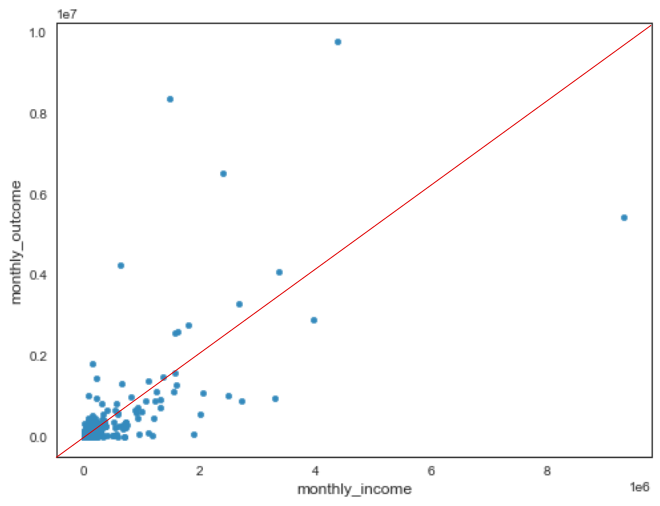
\includegraphics[scale=0.75]{Images/users_class_scatter.png}
    \caption{Users income}
    \label{fig:usersscatter}
\end{figure}\newpage

Finally, a correlation between the data in the table is generated to determine relations between columns. The result of that comparison is shown on figure \ref{fig:userscorr}.\vspace{3mm}

\begin{lstlisting}[language=python,caption = {Correlation of data}]
def plot_correlation_map( df ):
    corr = credit_reports.corr()
    _ , ax = plt.subplots( figsize =( 12 , 10 ) )
    cmap = sns.diverging_palette( 220 , 10 , as_cmap = True )
    _ = sns.heatmap(
        corr, 
        cmap = cmap,
        square=True, 
        cbar_kws={ 'shrink' : .9 }, 
        ax=ax, 
        annot = True, 
        annot_kws = { 'fontsize' : 12 }
    )
plot_correlation_map( credit_reports )
\end{lstlisting}

\begin{figure}[h!]
    \centering
    \includegraphics[scale=0.425]{Images/users_class_corr.png}
    \caption{Fields correlation}
    \label{fig:userscorr}
\end{figure}\newpage

\section{Data Preparation} 
Once we have a general idea of the data contained within the data set, it is necessary to clean the information and transform it in case it is needed.
The categorical values that result of importance can be assigned a ``dummy'' value in order to be identified and taken into consideration.

The original ``credit\_reports.csv'' presented codification errors while trying to read through accents on the account\_type and credit\_type columns. On the account\_opening- \_date, account\_closing\_date and worst\_delinquency\_date columns the dates where transformed to datetype, including the one with the ``0000-00-00'' format which was not recognized directly.
Finally four columns where added: institution\_cat, account\_ type\_cat, credit\_type\_cat and payment\_frequency\_cat; which correspond to institution, account\_type, credit\_type and payment\_frequency respectively. This fields are the non-categorical representation of those categorical values. The data types of this dataset are represented on the table \ref{tab:RCRtable}.\vspace{3mm}

\begin{lstlisting}[language=python,caption = {Data cleaning}]
clean_cr=credit_reports
clean_u=users
#Cleaning typos of accents
clean_cr=clean_cr.replace('"eacento"','e', regex=True)
clean_cr=clean_cr.replace('"iacento"','', regex=True)
clean_cr=clean_cr.replace('oacento','o', regex=True)
clean_cr=clean_cr.replace('uacento','u', regex=True)
#Unifying date format
clean_cr['account_opening_date'] = pd.to_datetime(clean_cr['account_opening_date'],format = "%x")
clean_cr['account_closing_date'] = pd.to_datetime(clean_cr['account_closing_date'],format = "%x")
clean_cr=clean_cr.replace('0000-00-00',None, regex=True)
clean_cr['worst_delinquency_date'] = pd.to_datetime(clean_cr['worst_delinquency_date'],format = "%x")
#Converting categorical to non-categorical
clean_cr["institution"] = clean_cr["institution"].astype('category')
clean_cr["institution_cat"]=clean_cr["institution"].cat.codes
clean_cr["account_type"] = clean_cr["account_type"].astype('category')
clean_cr["account_type_cat"]=clean_cr["account_type"].cat.codes
clean_cr["credit_type"] = clean_cr["credit_type"].astype('category')
clean_cr["credit_type_cat"]=clean_cr["credit_type"].cat.codes
clean_cr["payment_frequency"] = clean_cr["payment_frequency"].astype('category')
clean_cr["payment_frequency_cat"]=clean_cr["payment_frequency"].cat.codes
#Saving clean dataset
clean_cr.to_csv("clean_credit_records.csv",encoding='utf-8')
#Reduced dataset
reduced_cr=clean_cr
reduced_cr=reduced_cr.drop(columns=['institution','account_type','credit_type','total_credit_payments','payment_frequency'])
reduced_cr.to_csv("reduced_credit_records.csv",encoding='utf-8')
\end{lstlisting}\newpage


% Table generated by Excel2LaTeX from sheet 'reduced'
\begin{table}[h!]
  \centering
  \caption{Clean and reduced credit registers dataset}
    \begin{tabular}{|l|c|}
    \hline
    \rowcolor[rgb]{ .631,  .325,  .725} \multicolumn{1}{|c|}{\textcolor[rgb]{ 1,  1,  1}{Variable}} & \textcolor[rgb]{ 1,  1,  1}{Type of variable} \\
    \hline
    \multicolumn{1}{|c|}{user\_id} & int64 \\
    \hline
    amount\_to\_pay\_next\_payment & float64 \\
    \hline
    account\_opening\_date & datetime64[ns] \\
    \hline
    account\_closing\_date & datetime64[ns] \\
    \hline
    maximum\_credit\_amount & float64 \\
    \hline
    current\_balance & float64 \\
    \hline
    credit\_limit & float64 \\
    \hline
    past\_due\_balance & float64 \\
    \hline
    number\_of\_payments\_due & float64 \\
    \hline
    worst\_delinquency & float64 \\
    \hline
    worst\_delinquency\_date & datetime64[ns] \\
    \hline
    worst\_delinquency\_past\_due\_balance & float64 \\
    \hline
    institution\_cat & int8 \\
    \hline
    account\_type\_cat & int8 \\
    \hline
    credit\_type\_cat & int8 \\
    \hline
    payment\_frequency\_cat & int8 \\
    \hline
    \end{tabular}%
  \label{tab:RCRtable}%
\end{table}\newpage






\section{Modeling}
In this stage we will get the clients that are trusted to get a loan. First, we start discarding the clients by some set of rules.\\
\textbf{Rule 1:} Every user that was classidfied with '0' in users.csv is discarded\\
\textbf{Rule 2:} Every user which outcome is higher than its income is discarded\\
\textbf{Rule 3:} Only users that passed previous knockout rules remain on the reduced credit reports\\
\textbf{Rule 4:} Worst delinquency lower than 10\\

\begin{lstlisting}[language=python,caption = {Knock-out rules}]
#Modeling
#Knockout rule 1: Every user that was classidfied with '0' in users.csv is discarded 
fil_users=users[users['class'] == 1]
#Knockout rule 2: Every user which outcome is higher than its income is discarded
fil_users=fil_users[fil_users.monthly_income.gt(fil_users.monthly_outcome)] 
#Knockout rule 3: Only users that passed previous knockout rules remain on the reduced credit reports
fil_cr=reduced_cr[reduced_cr.user_id.isin(fil_users.id)]
fil_cr.to_csv("kickout_credit_records.csv",encoding='utf-8')
#Knockout rule 4: Worst delinquency lower than 10
gp_cr=fil_cr.groupby('user_id').sum('worst_delinquency')
gp_cr=gp_cr[gp_cr['worst_delinquency']<10]
gp_cr.to_csv("Users_kickout_pass.csv",encoding='utf-8')

gp_cr2=pd.read_csv("Users_kickout_pass.csv",encoding='utf-8')
m_dset=fil_cr[fil_cr.user_id.isin(gp_cr2.user_id)]
m_dset.to_csv("Model_Dataset.csv",encoding='utf-8')
\end{lstlisting}

This leaves us with a total of 175 clients to be recipient of loans. Out of this clients a linear regression can be used to determine loans. This dataset is saved as ``users\_kickout\_pass.csv''.\newpage


In order to analyze the information the relevant fields chosen were the ``user\_id'', to associate the loan generated, the ``account\_opening\_date'' retrieving the year from it and the ``maximum\_credit\_amount''. Once we have this information, we had two different approximations, a lineal regression, and the ordinary least squares.\vspace{3mm}

\begin{lstlisting}[language=python,caption = {Linear  regression}]
#Linear Regression 
import datetime as dt

m_dset2=m_dset[['user_id','account_opening_date','maximum_credit_amount']]
m_dset2['year'] = pd.DatetimeIndex(m_dset2['account_opening_date']).year
lr2_set=m_dset2[['user_id','year','maximum_credit_amount']]

#First, let's group the data by group
df_group = lr2_set.groupby('user_id')

#Then, we need to change the date to integer
from sklearn.model_selection import train_test_split

X = lr2_set[['year','user_id']]  # put your dates in here
y = lr2_set[['maximum_credit_amount']]

x_train, x_test, y_train, y_test = train_test_split(X, y)

model = LinearRegression()
model.fit(x_train, y_train)
print(model.score(x_train, y_train),model.score(x_test, y_test) )#check score
res_m=model.predict(x_test)
res_mm=res_m[8:23]
res_mm_prom=np.average(res_mm)
res_mm_prom
\end{lstlisting}\newpage

To test the results the user wit user\_id= '6', was employed. The value extracted from the lineal regression as a prediction is $\$$53,155 and the value obtained by the OLS is $\$$ 58,922. This achieve a difference of $\$$5,787.\vspace{3mm}

\begin{lstlisting}[language=python,caption = {OLS}]
#OLS
lr2_set.to_csv("OLS_data.csv",encoding='utf-8')
"""
Tomando como ejempplo los datos del usuario 6
2004	10831
2008	16304
2009	13493
2013	784
2014	40928
2015	69584
2016	25000
"""
#2004,2008,2009,2013,2014,2015,2016
six_x= np.array([1,5,6,10,11,12,13])
six_y= np.array([10831,16304,13493,784,40928,69584,25000])
six_xy= six_x*six_y
six_x2= six_x*six_x
six_y2= six_y*six_y

six_x_sum=np.sum(six_x)
six_y_sum=np.sum(six_y)
six_xy_sum=np.sum(six_xy)
six_x2_sum=np.sum(six_x2)
six_y2_sum=np.sum(six_y2)

six_x_prom=np.average(six_x)
six_y_prom=np.average(six_y)

#six_xy_sum-six_x[-1]
six_b=(six_xy_sum-(six_x[-1]*six_x_prom*six_y_prom))/(six_x2_sum-(six_x[-1]*six_x_prom*six_x_prom))
six_a=six_y_prom-(six_b*six_x_prom)

six_x_pred=np.array([14,15,16,17,18,19])
six_x_complete=np.concatenate((six_x,six_x_pred))

yp= six_a+(six_b*six_x_complete)
ypr=np.around(yp)
ypr=ypr.astype(int)

fig = plt.figure()
ax1 = fig.add_subplot(111)

ax1.plot(six_x,six_y)
ax1.plot(six_x_complete, ypr)
plt.show()
\end{lstlisting}\newpage

In the figure \ref{fig:OLS_graph}, 1 equals to 2004 on the x axis and 19 equals 2022, while the y axis represents the amount to be lend. Both of the models employed are useful to predict based on previous evidence, and contrasting them we can appreciate that produce somewhat similar results.


\begin{figure}[h!]
    \centering
    \includegraphics[scale=0.8]{Images/OLS_graph.png}
    \caption{OLS Graph}
    \label{fig:OLS_graph}
\end{figure}

\section{Evaluation}
In the case of the linear regression model it can be evaluated using the .score function and the corresponding sets, achieving a difference of approximately $1.67\times10^{-3}$. Meanwhile the OLS has an standard deviation of 14,187, which is elevated. 

The model was developed employing the year the account bank was opened, the maximum credit amount and the user id. The preliminary results seem to be a good first approximation instead of a final result. Further can be achieved in this section.\newpage

\section{Deployment}
The first question, ``Pick the best clients you will give a loan to, based on the model you created. It could be as complex as you decide (even as simpler as knock out rules), as long as the metrics support it'' can be partially answered by the knockout rules. Which are that this client is not under the bad client classification from the ``users.csv'' and that its income is greater than its outcome. Apart from this, users with a total delinquency lower than 10 for the total loans are selected.
After this we have a reduced dataset of 175 different clients that are suitable to get a loan. This can be found on the ``Users\_kickout\_pass.csv''.

The second question, ``Propose an amount to be lended to those clients and a term in which the loan will need to be paid back'', will be answered according to the user with "id = 6" ($\$$53,155 the amount to be lend), in this is case the payment frequency shall be monthly since it matches previous loan formats. The difference between income and outcome is  $\$$3,228 for this user. Considering half of this number, to have a margin and dividing it by 2, it results in monthly rates of $\$$1,644 that are equivalent to 32.3 $\approx$ 33 monthly payments.

The third question, ``Finally choose an annual interest rate the lended amount must have in order to be profitable'', has more to do with the economic reality of the country, and colsulting ``Indicadores Básicos de Créditos a las Pequeñas y Medianas
Empresas (PYMES)'' from Banxico\cite{"Banxico"}, an annual 12.8\% is granted, eventhough this rate was set for 2017 and a new rates are subject to being updated.
While researching, for more recent data, including some from Konfio, it was found that the for a \$500,000 loan, a 28\% was asigned. And this might be a closer approach to a real rate, leaving our monthly payments on $\$$2,104.32 pesos.



%%%%%%%%%%%%%%%%%%%%%%%%%%%%%%%%%%%%%%%%%%%%%%%%%%%%%%%%%%%%%%%%%%%%%%%%%%%%%%%%%%
\newpage
\bibliographystyle{IEEEtran}
\bibliography{bibtex}

% Aquí termina el documento
\end{document}